\documentclass[12pt]{article}

\usepackage[a4paper,margin=2.5cm]{geometry}
\usepackage{amsmath, amssymb, amsthm}
\usepackage{bm}
\usepackage{hyperref}
\usepackage{graphicx}
\usepackage{caption}
\usepackage{listings}
\usepackage{xcolor}
\usepackage{float}
\usepackage{placeins}
\graphicspath{{figures/}}

\lstdefinestyle{code}{
  basicstyle=\ttfamily\small,
  numbers=left,
  numberstyle=\tiny,
  numbersep=8pt,
  keywordstyle=\color{blue},
  commentstyle=\color{teal!70!black},
  stringstyle=\color{orange!70!black},
  showstringspaces=false,
  breaklines=true,
  frame=single,
  framerule=0.3pt,
  rulecolor=\color{black!15}
}
\lstset{style=code}

\title{REINFORCE Algorithm Tutorial}
\author{}
\date{\today}

\begin{document}
\maketitle

\section{Introduction}
REINFORCE, also known as Monte Carlo policy gradient, updates policy parameters using complete trajectory returns. It provides an unbiased estimator of the policy gradient by weighting log-probability gradients with observed returns, making it the foundational algorithm for policy gradient methods.

\section{Theory and Formulas}
\subsection{Monte Carlo Policy Gradient}
Given trajectories \(\tau\) sampled from policy \(\pi_\theta\), the REINFORCE gradient estimator is
\begin{equation}
\nabla_\theta J(\theta) = \mathbb{E}_{\tau \sim \pi_\theta}\Big[ \sum_{t=0}^{T-1} \nabla_\theta \log \pi_\theta(a_t\mid s_t)\, G_t \Big],
\end{equation}
where \(G_t = \sum_{k=t}^{T-1} \gamma^{k-t} r_{k+1}\) is the return from time \(t\).

\subsection{Baselines and Variance Reduction}
Adding a baseline \(b(s_t)\) retains unbiasedness while reducing variance:
\begin{equation}
\nabla_\theta J(\theta) = \mathbb{E}\Big[ \sum_{t} \nabla_\theta \log \pi_\theta(a_t\mid s_t)\, (G_t - b(s_t)) \Big].
\end{equation}
Typical choices include constant baselines, value-function estimates, or EMAs of returns.

\subsection{Algorithm Steps}
\begin{enumerate}
  \item Collect trajectories by rolling out \(\pi_\theta\).
  \item Compute returns \(G_t\) for each time step.
  \item Update parameters with gradient ascent: \(\theta \leftarrow \theta + \alpha \sum_t \nabla_\theta \log \pi_\theta(a_t\mid s_t) (G_t - b(s_t))\).
  \item Optionally update the baseline estimate.
\end{enumerate}
Because REINFORCE relies on full trajectory returns, it exhibits higher variance than actor-critic methods but is simple and unbiased.

\section{Applications and Tips}
\begin{itemize}
  \item \textbf{Episodic tasks}: environments with moderate episode length and sparse rewards.
  \item \textbf{Curriculum learning}: warm-start more advanced actor-critic algorithms.
  \item \textbf{Discrete policies}: categorical action spaces or parameterized bandits.
  \item \textbf{Best practices}: normalize returns within batches, use baselines, tune learning rate carefully, and consider reward-to-go to reduce variance.
\end{itemize}

\section{Python Practice}
The script \texttt{gen\_reinforce\_figures.py} trains a softmax policy in a grid-world with terminal rewards using REINFORCE and a moving-average baseline. It records episodic returns and state visitation frequencies under the learned policy.
\begin{lstlisting}[language=Python,caption={Excerpt from gen_reinforce_figures.py}]
returns = compute_returns(rewards, gamma)
for (state, action), G_t in zip(trajectory, returns):
    probs = softmax(theta[state])
    grad = -probs
    grad[action] += 1.0
    baseline[state] += baseline_lr * (G_t - baseline[state])
    theta[state] += alpha * grad * (G_t - baseline[state])
\end{lstlisting}

\section{Result}
\begin{figure}[H]
  \centering
  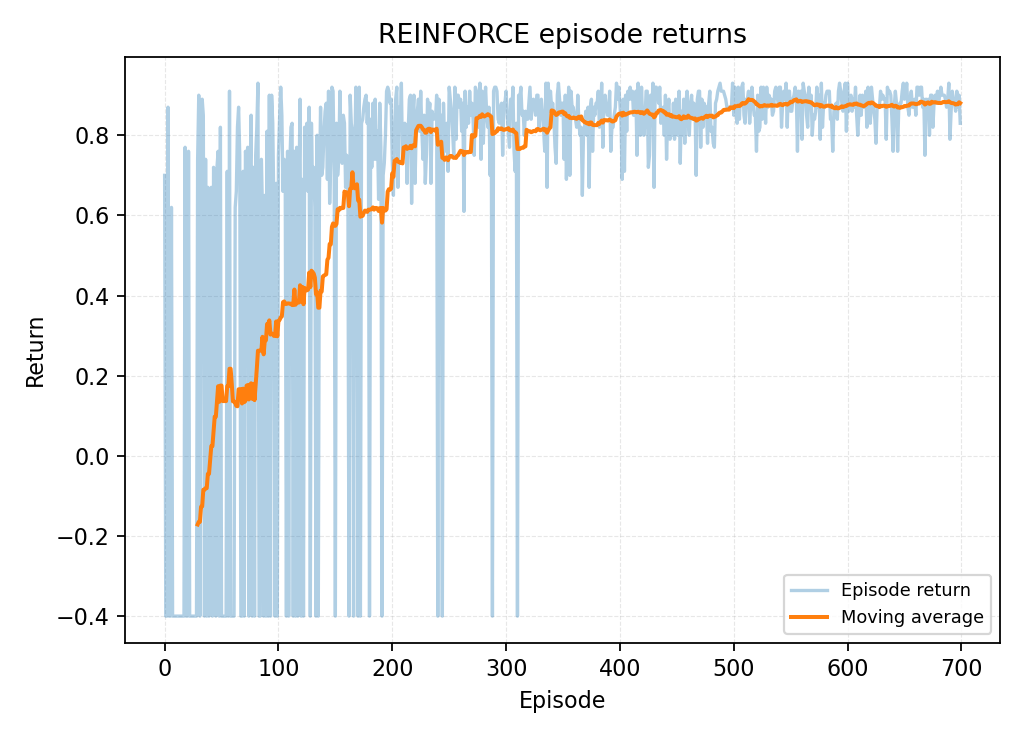
\includegraphics[width=0.8\linewidth]{reinforce_returns.png}
  \caption{REINFORCE episode returns with moving average smoothing}
  \label{fig:reinforce_returns}
\end{figure}

\begin{figure}[H]
  \centering
  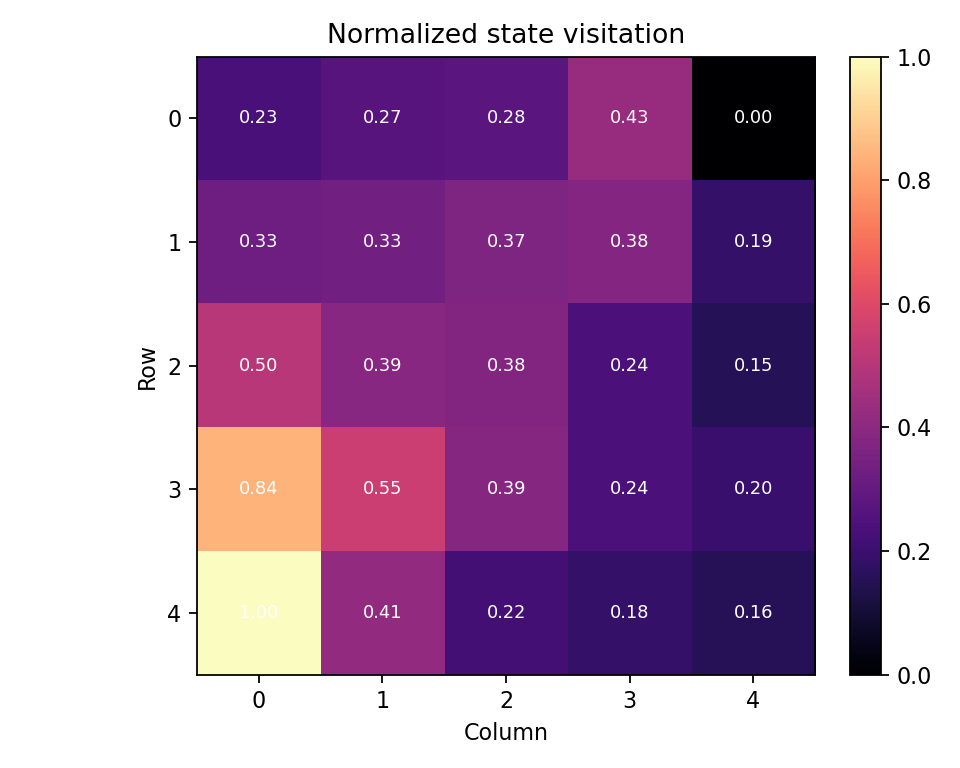
\includegraphics[width=0.82\linewidth]{reinforce_state_visitation.png}
  \caption{State visitation heatmap after training, highlighting preferred trajectories}
  \label{fig:reinforce_state_visitation}
\end{figure}

\FloatBarrier
\section{Summary}
REINFORCE offers a simple, unbiased policy gradient estimator but requires careful variance reduction and learning-rate tuning. Baselines, reward normalization, and batch averaging help stabilize learning. The grid-world example shows returns improving as the policy concentrates on efficient paths.

\end{document}